% ============================================================
% file: forward_reverse_ad.tex
% Forward-mode and reverse-mode AD for Jacobian construction
% ============================================================

\documentclass{standalone}
\usepackage{tikz}
\usetikzlibrary{arrows.meta, positioning, calc}
\usepackage{amsmath}
\usepackage{amssymb}

\begin{document}

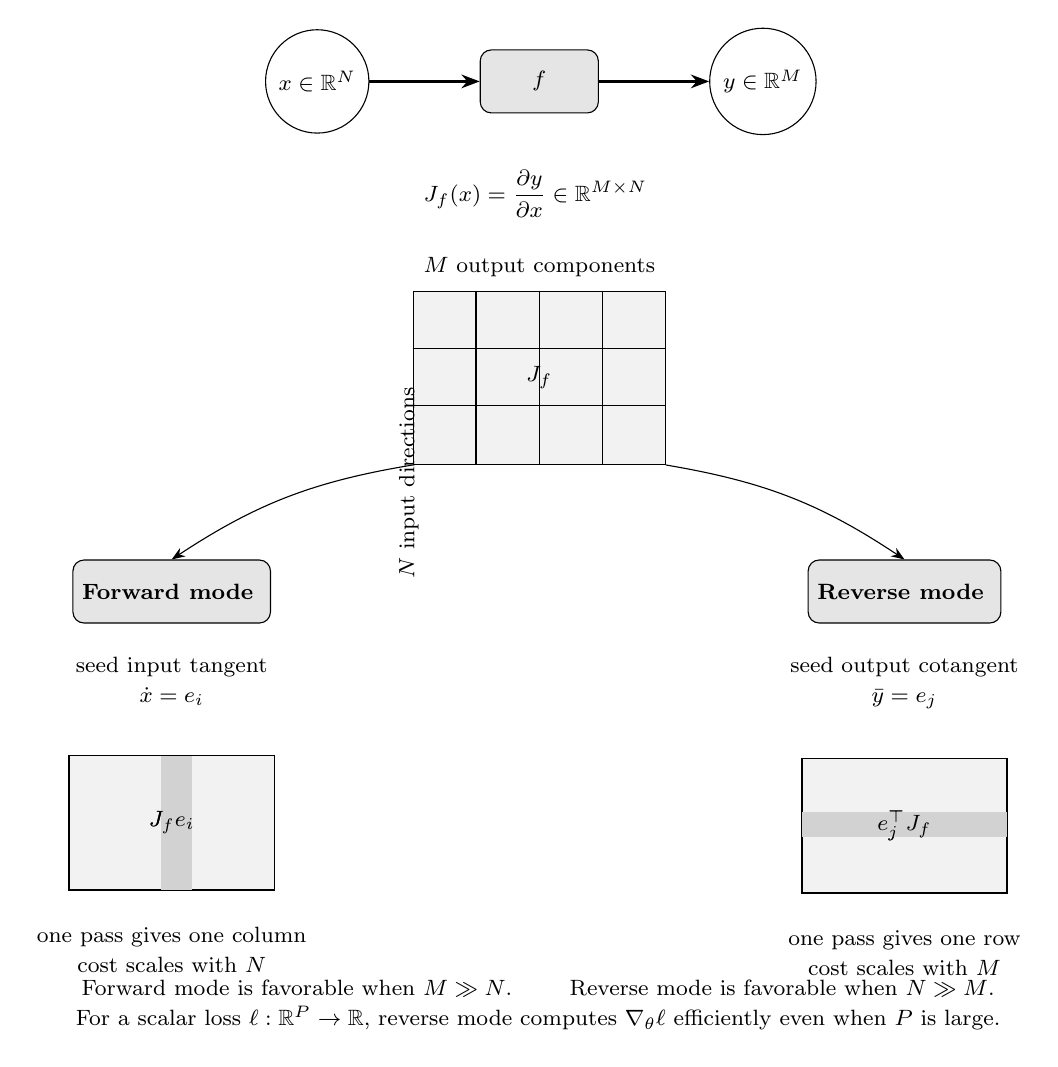
\begin{tikzpicture}[
  block/.style={
    rectangle,
    draw,
    rounded corners,
    minimum width=1.5cm,
    minimum height=0.8cm,
    align=center,
    fill=gray!20
  },
  var/.style={
    circle,
    draw,
    minimum width=0.9cm,
    minimum height=0.9cm,
    align=center,
    fill=white!20
  },
  mat/.style={
    rectangle,
    draw,
    minimum width=3.2cm,
    minimum height=2.2cm,
    align=center,
    fill=gray!10
  },
  note/.style={
    align=center
  },
  every node/.style={font=\footnotesize},
  arrow/.style={-Stealth, thick},
  lightarrow/.style={-Stealth, thin},
  dashedarrow/.style={-Stealth, thick, dashed}
]

% ============================================================
% Top: function and Jacobian
% ============================================================

\node[var] (x) {$x\in\mathbb R^N$};
\node[block, right=1.4cm of x] (f) {$f$};
\node[var, right=1.4cm of f] (y) {$y\in\mathbb R^M$};

\draw[arrow] (x) -- (f);
\draw[arrow] (f) -- (y);

\node[note, below=0.6cm of f] (jaclabel) {
$\displaystyle J_f(x)=\frac{\partial y}{\partial x}\in\mathbb R^{M\times N}$
};

% ============================================================
% Middle: Jacobian matrix
% ============================================================

\node[mat, below=0.8cm of jaclabel] (J) {$J_f$};

% Matrix grid lines
\draw ($(J.north west)!0.25!(J.north east)$) -- ($(J.south west)!0.25!(J.south east)$);
\draw ($(J.north west)!0.50!(J.north east)$) -- ($(J.south west)!0.50!(J.south east)$);
\draw ($(J.north west)!0.75!(J.north east)$) -- ($(J.south west)!0.75!(J.south east)$);

\draw ($(J.north west)!0.33!(J.south west)$) -- ($(J.north east)!0.33!(J.south east)$);
\draw ($(J.north west)!0.66!(J.south west)$) -- ($(J.north east)!0.66!(J.south east)$);

\node[note, above=0.05cm of J] {$M$ output components};
\node[note, rotate=90, left=0.05cm of J] {$N$ input directions};

% ============================================================
% Bottom-left: forward mode
% ============================================================

\node[block, below left=1.2cm and 1.8cm of J] (fwdtitle) {
\textbf{Forward mode}
};

\node[note, below=0.3cm of fwdtitle] (fwdtext) {
seed input tangent\\[0.05cm]
$\dot x=e_i$
};

\node[mat, below=0.5cm of fwdtext, minimum width=2.6cm, minimum height=1.7cm] (Jcol) {$J_f e_i$};

% Highlight a column
\fill[gray!35] ($(Jcol.north west)!0.45!(Jcol.north east)$) rectangle ($(Jcol.south west)!0.60!(Jcol.south east)$);
\node at (Jcol.center) {$J_f e_i$};

% Redraw border after fill
\draw (Jcol.north west) rectangle (Jcol.south east);

\node[note, below=0.35cm of Jcol] {
one pass gives one column\\[0.05cm]
cost scales with $N$
};

% ============================================================
% Bottom-right: reverse mode
% ============================================================

\node[block, below right=1.2cm and 1.8cm of J] (revtitle) {
\textbf{Reverse mode}
};

\node[note, below=0.3cm of revtitle] (revtext) {
seed output cotangent\\[0.05cm]
$\bar y=e_j$
};

\node[mat, below=0.5cm of revtext, minimum width=2.6cm, minimum height=1.7cm] (Jrow) {$e_j^\top J_f$};

% Highlight a row
\fill[gray!35] ($(Jrow.north west)!0.40!(Jrow.south west)$) rectangle ($(Jrow.north east)!0.58!(Jrow.south east)$);
\node at (Jrow.center) {$e_j^\top J_f$};

% Redraw border after fill
\draw (Jrow.north west) rectangle (Jrow.south east);

\node[note, below=0.35cm of Jrow] {
one pass gives one row\\[0.05cm]
cost scales with $M$
};

% ============================================================
% Arrows from Jacobian to modes
% ============================================================

\draw[lightarrow] (J.south west) to[bend right=12] (fwdtitle.north);
\draw[lightarrow] (J.south east) to[bend left=12] (revtitle.north);

% ============================================================
% Bottom comparison note
% ============================================================

\node[note, below=1.0cm of $(Jcol.south)!0.5!(Jrow.south)$] {
Forward mode is favorable when $M\gg N$. \qquad
Reverse mode is favorable when $N\gg M$.\\[0.05cm]
For a scalar loss $\ell:\mathbb R^P\to\mathbb R$, reverse mode computes
$\nabla_\theta \ell$ efficiently even when $P$ is large.
};

\end{tikzpicture}

\end{document}